\documentclass[12pt]{article}
\usepackage{caption}
\usepackage{subcaption}
\usepackage{graphicx}
\graphicspath{ {Imagens/} }
\usepackage{geometry}
\usepackage{pdfpages}
\usepackage{array}
\usepackage{amsmath}
\usepackage{url}
\usepackage[portuguese]{babel}
\usepackage{float}


\tolerance=1
\emergencystretch=\maxdimen
\hyphenpenalty=10000
\hbadness=10000

%opening
\title{Exercícios de Fixação de Conceitos 3 - EFC3 - IA048}
\author{Marcelo Eduardo Pederiva RA: 122580}
\date{}
\geometry{total={210mm,297mm},
	left=20mm,right=20mm,
	bindingoffset=10mm, top=0mm,bottom=20mm}

\begin{document}

\maketitle
\vfill
\section*{Parte 1 - Classificação Binária com redes MLP}
\subsection*{a)}



\begin{figure}[H]
	\centering
	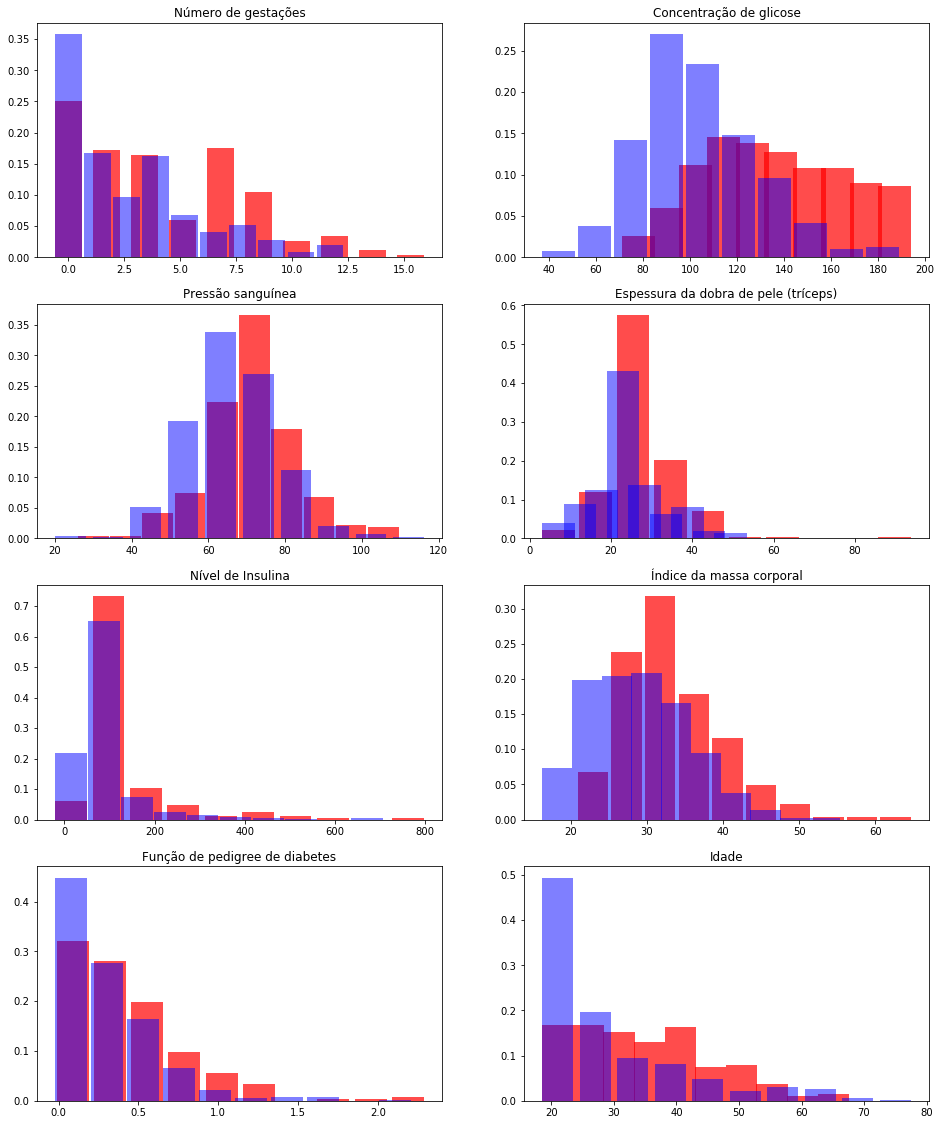
\includegraphics[width=0.8\linewidth]{Imagens/hist.png}
	\caption{Histogramas, as barras vermelhas representam diagnostico positivo para diabetes e as barras azuis negativo.}
	\label{fig:hist}
\end{figure}

\newgeometry{left=3cm, right = 2cm, textwidth=12cm,top=1.5cm,bottom=2cm,heightrounded}

Inicialmente, para a análise dos dados, foi observado um desbalanceamento entre a quantidade de pessoas com diagnostico positivo para diabetes e as diagnosticadas negativamente. No qual, a quantidade de dados de pessoas diagnosticadas sem diabetes representam quase o dobro da quantidade de dados classificados de forma contrária. Dessa forma, para observar o a relevância de cada atributo para a classificação de cada classe, foi feito uma normalização do total de cada classe para cada atributo.  Em outras palavras, o histograma apresentado pela Figura \ref{fig:hist} demonstra, em seu eixo y, porcentagem de pessoas para cada atributo.

Como podemos observar pelos dados, o problema apresenta um grande desafio, uma vez que os atributos não apresentam grandes diferenças para representação de um tipo de diagnostico. Podemos observar que a concentração de glicose representa um dos principais fatores de distinção entre as classes. Já o histograma do Nivel de Insulina demonstra um resultado próximo dentre as duas classificações.

Entretanto, os histogramas se diferenciam em alguns casos, como Idade e Número de Gestações. Nestes atributos, o histograma de uma categoria apresenta um pico em uma região, enquanto a outra possui uma distribuição não acentuada. Esses casos provavelmente irão ter grande relevância para a classificação correta do diagnostico apos o treinamento da MLP.

\subsection*{b)}

Para o treinamento da Máquina, inicialmente foi feito uma normalização dos dados de pela técnica Min-Max:

\begin{equation}
X' = \frac{X - \min(X)}{\max(X)-\min(X)}
\end{equation}

A seguir, para o treinamento foi separado os dados entre dados de treinamento e dados de validação (\textit{Holdout}). Para isso, levando em conta o desbalanceamento das classes, foi separado 20\% dos dados diagnosticados positivamente mais 20\% dos dados contrários, para validação. Da mesma forma, foi somado os 80\% de cada classe como base de dados de treinamento. 

Após o embaralhamento dos dados, foi feito o treinamento de uma MLP com 1 camada intermediária. Nessa etapa, foi variado os números de neurônios na camada intermediária dentre os seguintes valores: 
\begin{center}
	16 | 32 | 64 | 128 | 256 | 512 | 1024 | 2048 | 4096 | 8192
\end{center}

O treinamento de todos modelos foi feito com o cálculo do \textit{loss} = \textit{"sparse\_categorical\_crossentropy"}, o otimizador = "adam", \textit{bach\_size} = 64, \textit{epochs} = 200 e  um "\textit{callback}" de \textit{EarlyStopping} monitorando o mínimo do "\textit{loss\_validation}". Dessa forma, o \textit{callback} buscou interromper o treinamento para que o modelo apresentasse o mínimo de \textit{overfitting}.

\pagebreak
Após o treinamento encontramos uma variação de acurácia e do \textit{loss} dos dados de validação de acordo com cada modelo.


\begin{figure}[H]
	\begin{subfigure}{0.49\linewidth}
		\centering
		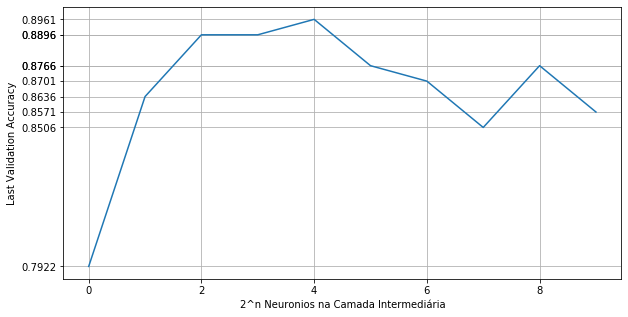
\includegraphics[width=\linewidth]{Imagens/best_acc_models.png}
		\caption{Acurácia frente aos dados de Validação de acordo com cada modelo.}
		\label{fig:best_acc_models}
	\end{subfigure}
	\hfill
	\begin{subfigure}{0.49\linewidth}
		\centering
		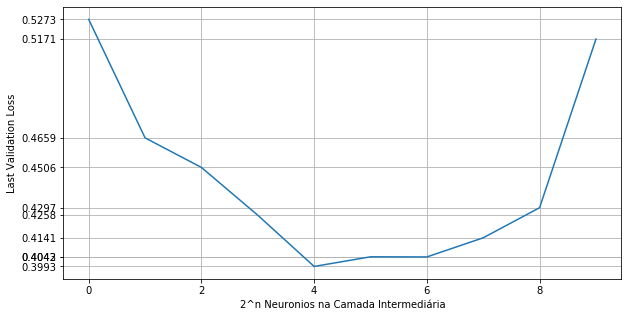
\includegraphics[width=\linewidth]{Imagens/best_loss_models.png}
		\caption{Loss frente aos dados de Validação de acordo com cada modelo.}
		\label{fig:best_loss_models}
	\end{subfigure}
	\caption{Comparação dos modelos MLP.}
	\label{fig:comp_mlp}
\end{figure}


Como podemos observar na Figura \ref{fig:comp_mlp}, o modelo que utilizou $2^4$ (256) neurônios na camada intermediária apresentou o melhor resultado, tanto nos valores de acurácia, quanto nos dados de \textit{loss}.

\subsection*{c)}

Com o número de neurônios definidos no item b) utilizamos o modelo com 256 neurônios para treinar em 400 épocas (\textit{epochs}). Com os outros parâmetros definidos da mesma forma, neste momento o \textit{callback} utilizado foi o de \textit{ModelCheckpoint}, o qual permite um salvamento dos pesos treinados cada vez que o valor de \textit{loss\_validation} diminuísse (ou o valor de \textit{acuraccy\_validation} aumentasse), tendo assim os pesos com o epoch que permitiu o mínimo de \textit{overfitting}, ou máximo de acurácia.

Na Figura \ref{fig:acc_evolution_loss} temos a evolução do treino deste modelo.
\begin{figure}[H]
	\centering
	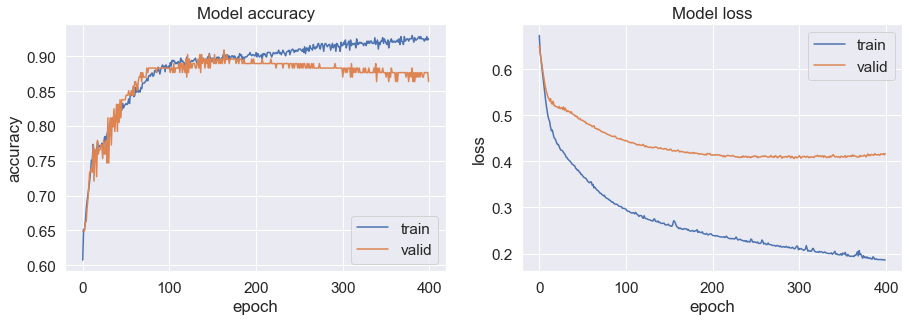
\includegraphics[width=\linewidth]{Imagens/acc_evolution_loss.png}
	\caption{Evolução do treinamento do MLP.}
	\label{fig:acc_evolution_loss}
\end{figure}

Podemos observar que a acurácia de validação se mantém constante após, aproximadamente, a época 150, enquanto a acurácia de treinamento continua subindo. Este mesmo fenômeno pode ser observado com as curvas de \textit{loss}, com o \textit{loss} de treinamento diminuindo. Esse contraste entre os dois valores de acurácia demonstra o máximo que o treinamento alcançou antes de apresentar \textit{overfitting}.

Com o \textit{callback} (ModelCheckpoint) salvando os pesos no menor \textit{loss\_validation} e maior \textit{accuracy\_validation}, garantimos o salvamento dos pesos que represente o melhor modelo em acurácia ou \textit{loss} frente aos dados de validação. 

Assim, para a análise dos modelos em diferentes aspectos. O treinamento salvou o peso que apresentasse o menor \textit{loss} e a \textit{maior} acurácia com os dados de validação.

O modelo apresentou o seguinte resultado:

\begin{center}
	\textbf{Minimum Loss Checkpoint}: 
	\hspace{80px}
	Best Accuracy: 88.31 \% \hfill
	Loss : 0.406362 
	
	\textbf{Maximum Accuracy Checkpoint}: 
	\hspace{48px}
	Best Accuracy: 90.26 \% \hfill
	Loss : 0.426401
\end{center}

É interessante observar como os resultados divergem entre a melhor acurácia e o melhor \textit{loss}, demonstrando que para obter um modelo com o menor \textit{overfitting} não será, necessariamente, o modelo com a maior acurácia.

Por fim, temos a Matriz de Confusão destes dois modelos. Ambos apresentam resultados bem próximos, com um maior número de acerto dos casos negativos devido aos desbalanceamento dos dados.


\begin{figure}[H]
	\begin{subfigure}{0.49\linewidth}
		\centering
		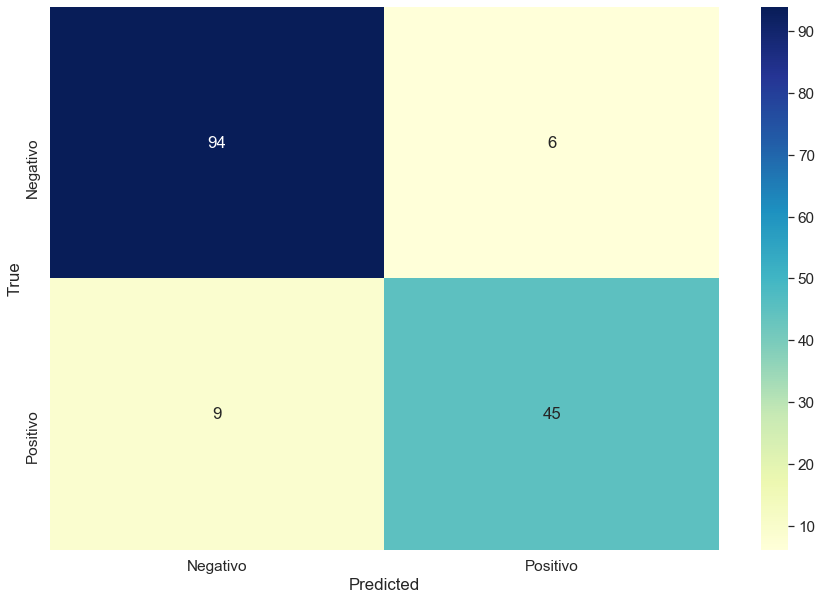
\includegraphics[width=\linewidth]{Imagens/conf_max_acc.png}
		\caption{Maximum Accuracy Checkpoint.}
		\label{fig:conf_max_acc}
	\end{subfigure}
	\hfill
	\begin{subfigure}{0.49\linewidth}
		\centering
		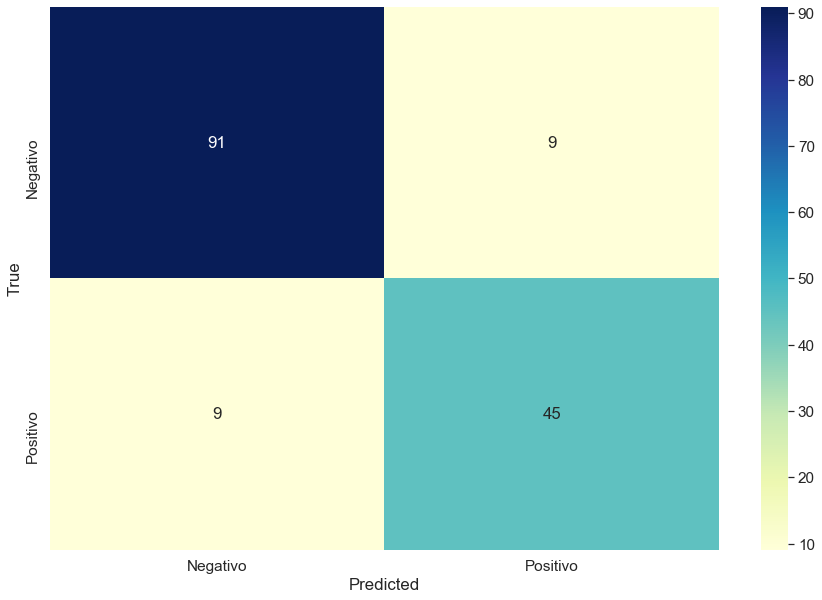
\includegraphics[width=\linewidth]{Imagens/conf_min_loss.png}
		\caption{Minimum Loss Checkpoint.}
		\label{fig:conf_min_loss}
	\end{subfigure}
	\caption{MLPs treinadas.}
	\label{fig:comp_mlp_f}
\end{figure}

\pagebreak
\section*{Parte 2 - MNIST, MLP e CNN}


\subsection*{a)}

Para a análise das MLPs com quantidades diferentes de camadas, foi definido os seguintes modelos:

\textbf{Modelo 1:}\\
tf.keras.layers.Flatten(),\\ \color{red}
tf.keras.layers.Dense(512, activation='relu'),\\ \color{black}
tf.keras.layers.Dense(10, activation='softmax')\\

\textbf{Modelo 2:}\\
tf.keras.layers.Flatten(),\\ \color{red}
tf.keras.layers.Dense(512, activation='relu'),\\
tf.keras.layers.Dropout(0.5),\\ \color{black}
tf.keras.layers.Dense(10, activation='softmax')\\

\textbf{Modelo 3:}\\
tf.keras.layers.Flatten(),\\ \color{red}
tf.keras.layers.Dense(1024, activation=tf.nn.relu),\\
tf.keras.layers.Dropout(0.5),\\
tf.keras.layers.Dense(256, activation=tf.nn.relu),\\ \color{black}
tf.keras.layers.Dense(10, activation='softmax')\\


\textbf{Modelo 4:}\\
tf.keras.layers.Flatten(),\\ \color{red}
tf.keras.layers.Dense(1024, activation=tf.nn.relu),\\
tf.keras.layers.Dropout(0.5),\\
tf.keras.layers.BatchNormalization(),\\
tf.keras.layers.Dense(256, activation=tf.nn.relu),\\ \color{black}
tf.keras.layers.Dense(10, activation='softmax')\\

Modelo 1,2 e 3 com 1,2,3 camadas intermediárias, respectivamente. Para observação do \textit{BatchNormalization}, foi implementado um 4° modelo onde foi adicionado 1 camada a mais, de \textit{BatchNormalization}, no meio das camadas anteriores, apenas para observar se este modelo irá apresentar um desempenho melhor que a encontrada no modelo 3.

Todos os modelos foram treinados com os mesmos parâmetros:\\
| Otimizador = "adam"\\
| Loss = "sparse\_categorical\_crossentropy"\\
| epochs=10\\
| batch\_size = 64 \\
| callback = EarlyStopping, interrompendo o treinamento no mínimo \textit{loss\_validation}\\
\pagebreak

Com todos modelos treinados, podemos observar o desempenho de cada um deles de acordo com suas máximas acurácias e mínimos valores de \textit{loss}, frente aos dados de teste.

\begin{figure}[H]
	\begin{subfigure}{0.49\linewidth}
		\centering
		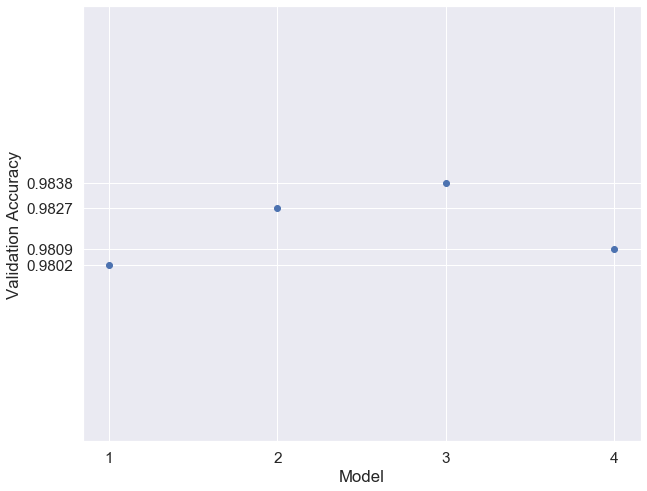
\includegraphics[width=\linewidth]{Imagens/mlp_acc.png}
		\caption{Acurácia de cada modelo.}
		\label{fig:mlp_acc}
	\end{subfigure}
	\hfill
	\begin{subfigure}{0.49\linewidth}
		\centering
		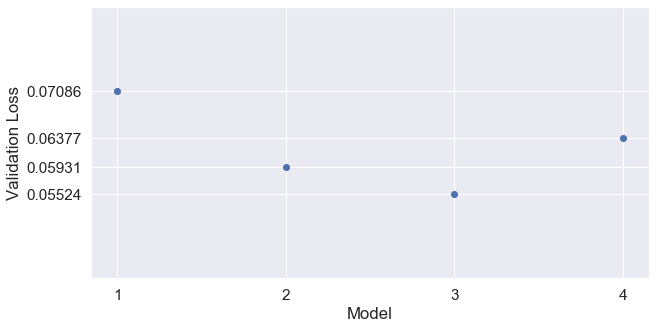
\includegraphics[width=\linewidth]{Imagens/mlp_loss.png}
		\caption{Loss de cada modelo.}
		\label{fig:mlp_loss}
	\end{subfigure}
	\caption{Comparação dos modelos.}
	\label{fig:comp_models}
\end{figure}

Observamos que a implementação do Dropout resultou num aumento de performance do modelo 1 para o 2 e o aumento de neuronios junto com a implementação de outra camada com 256 neurônios melhorou ainda mais esta performance. O 4° modelo, com a implementação do BatchNormalization apresentou um decaimento na performance do modelo 3. Sendo assim, o Modelo 3 se destacou dentre os outros pela maior acurácia e menor valor de \textit{loss}.

\begin{figure}[H]
	\centering
	\begin{subfigure}{0.4\linewidth}
		\centering
		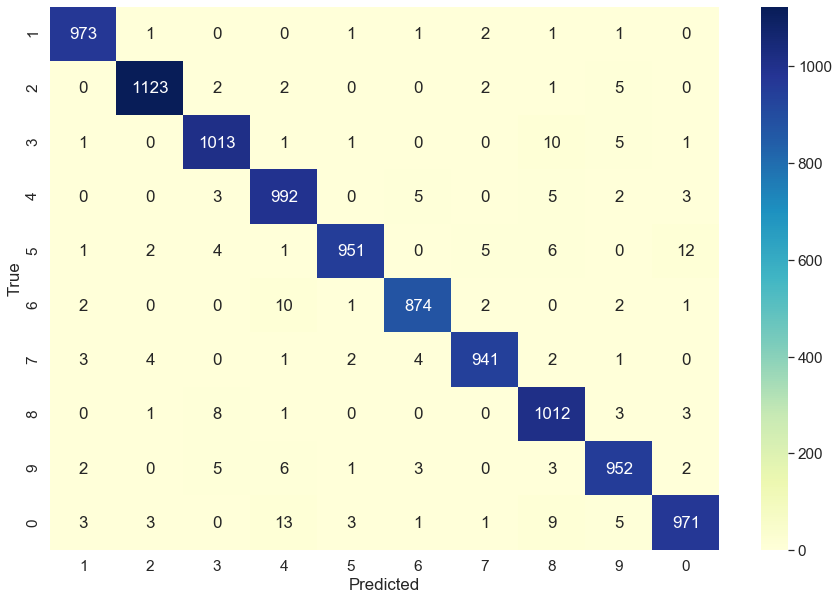
\includegraphics[width=\linewidth]{Imagens/mlp_model1_conf.png}
		\caption{Modelo 1.}
		\label{fig:mlp_model1_conf}
	\end{subfigure}
	\begin{subfigure}{0.4\linewidth}
		\centering
		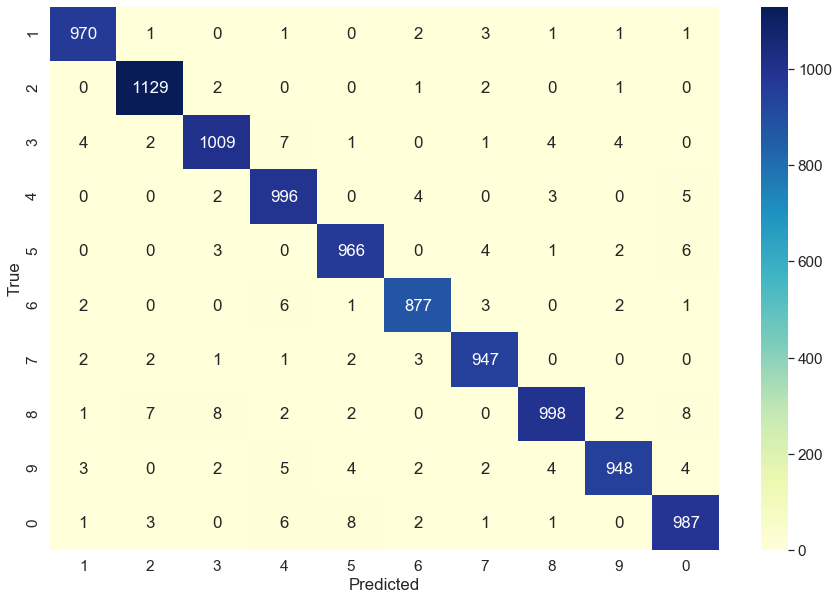
\includegraphics[width=\linewidth]{Imagens/mlp_model2_conf.png}
		\caption{Modelo 2.}
		\label{fig:mlp_model2_conf}
	\end{subfigure}

	\begin{subfigure}{0.4\linewidth}
		\centering
		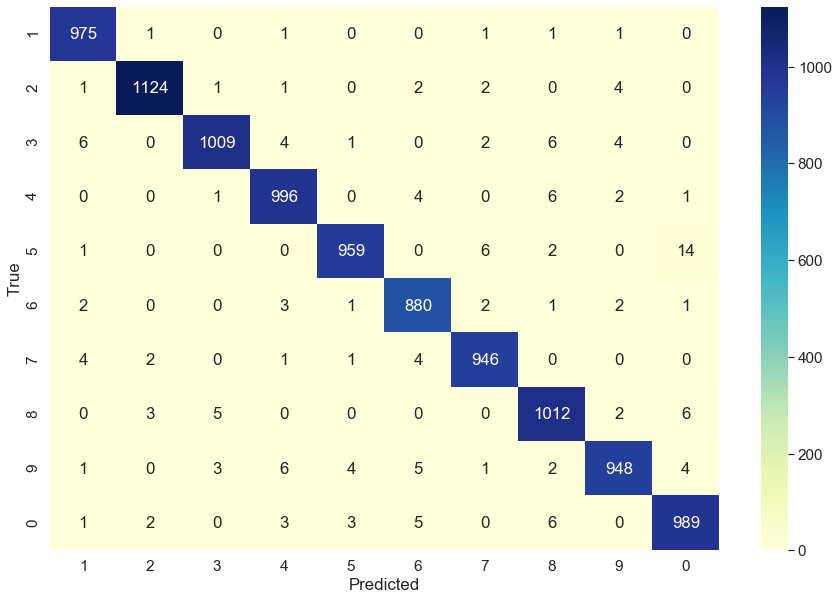
\includegraphics[width=\linewidth]{Imagens/mlp_model3_conf.png}
		\caption{Modelo 3.}
		\label{fig:mlp_model3_conf}
	\end{subfigure}
		\begin{subfigure}{0.4\linewidth}
		\centering
		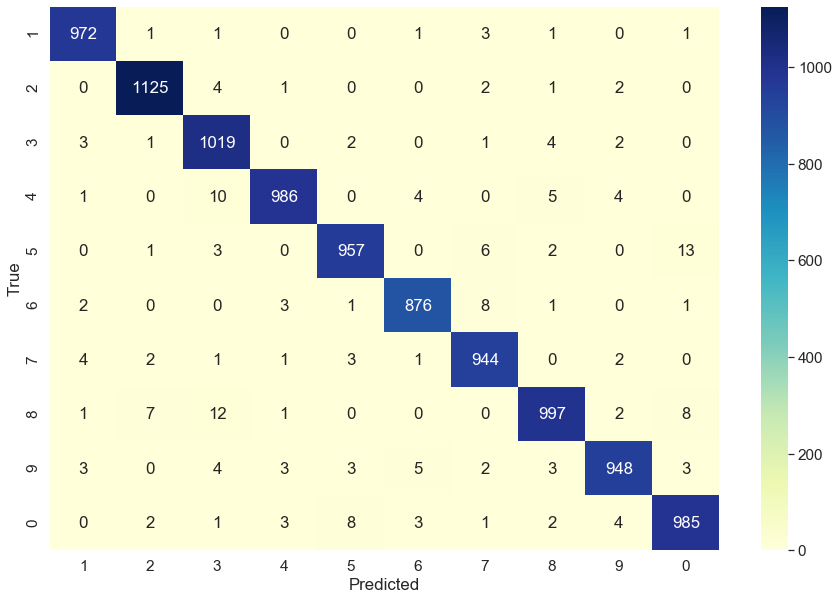
\includegraphics[width=\linewidth]{Imagens/mlp_model4_conf.png}
		\caption{Modelo 4.}
		\label{fig:mlp_model4_conf}
	\end{subfigure}
	\caption{Comparação dos modelos.}
	\label{fig:conf_models}
\end{figure}

Observamos pelas Matrizes de Confusão, que o Modelo 3 possui um desempenho muito próximo das demais. Apesar de não apresentar o maior número de acertos em todas classes, o modelo manteve uma maior precisão geral comparada com os outros.

\subsection*{b)}

\subsubsection*{1)}

Nesta etapa, iremos implementar uma CNN. O modelo possui a seguinte arquitetura:\\
\\
Conv2D(\color{red}number\color{black}, kernel\_size=(\color{red}size\color{black}, \color{red}size\color{black}), activation='relu', input\_shape=(28, 28, 1))\\
MaxPooling2D(pool\_size=(2, 2))\\
Flatten()\\
Dense(10, activation='softmax') \\

Neste item, utilizaremos um tamanho fixo de \textit{kernel}, \textit{size} = 2, e iremos variar a quantidade de \textit{kernels} (\textit{number}) presentes na camada convolucional. As quantidades serão variadas dentro dos seguintes valores:

\begin{center}
	32 | 64 | 128 | 256 | 512 | 1024
\end{center}

Para o treinamento foi utilizado os mesmos parâmetros do item a).

\begin{figure}[H]
	\centering
	\begin{subfigure}{0.65\linewidth}
		\centering
		\includegraphics[width=\linewidth]{Imagens/q2/qk_acc_var.png}
		\caption{Acurácia de cada modelo.}
		\label{fig:qk_acc_var}
	\end{subfigure}

	\begin{subfigure}{0.65\linewidth}
		\centering
		\includegraphics[width=\linewidth]{Imagens/q2/qk_loss_var.png}
		\caption{Loss de cada modelo.}
		\label{fig:qk_loss_var}
	\end{subfigure}
	\caption{Comparação das quantidades de \textit{kernels}.}
	\label{fig:comp_k}
\end{figure}

Como podemos observar na Figura \ref{fig:comp_k}, os modelos que apresentaram melhores acurácias não apresentaram os melhores valores de \textit{loss}. Entretanto, os valores de \textit{loss} com até 256 \textit{kernels} tiveram uma baixa variação. Além disso, observando os valores de acurácia, o modelo que usou 256 \textit{kernels} se mostrou o mais preciso.

Levando em conta os dois fatores, foi escolhido o modelo com 256 \textit{kernels}, pela relação geral entre a acurácia e o valor de \textit{loss}.

\subsubsection*{2)}

Tendo definido a quantidade de \textit{kernels}, fixamos este parâmetro (\textit{number} = 256) e variamos o tamanho dos \textit{kernels}(\textit{size}) entre os valores:

\begin{center}
	1 | 2 | 3 | 4 | 5
\end{center}

Usando os mesmos parâmetros de treinamento do item anterior, obtemos o seguinte resultado.

\begin{figure}[H]
	\centering
	\begin{subfigure}{0.65\linewidth}
		\centering
		\includegraphics[width=\linewidth]{Imagens/q2/nk_acc_var.png}
		\caption{Acurácia de cada modelo.}
		\label{fig:nk_acc_var}
	\end{subfigure}
	
	\begin{subfigure}{0.65\linewidth}
		\centering
		\includegraphics[width=\linewidth]{Imagens/q2/nk_loss_var.png}
		\caption{Loss de cada modelo.}
		\label{fig:nk_loss_var}
	\end{subfigure}
	\caption{Comparação dos tamanhos do \textit{kernel}.}
	\label{fig:comp_nk}
\end{figure}

O desempenho do aumento do tamanho do \textit{kernel} apresentou uma curva, onde o máximo de acurácia e mínimo de erro se manifestou no mesmo modelo, quando foi utilizado o $size = 4$. 

Sendo assim, este parâmetro foi escolhido para seguir com a atividade.

\subsection*{c)}

Utilizando os resultados obtidos pelos itens anteriores, montamos a seguinte CNN:\\
\\
Conv2D(\color{red}256\color{black}, kernel\_size=(\color{red}4\color{black}, \color{red}4\color{black}), activation='relu', input\_shape=(28, 28, 1))\\
MaxPooling2D(pool\_size=(2, 2))\\
Flatten()\\
Dense(10, activation='softmax') \\

Com o treinamento monitorando o mínimo \textit{loss\_validation}, o modelo apresentou o seguinte desempenho:

\begin{figure}[H]
	\centering
	\includegraphics[width=\linewidth]{Imagens/q2/best_cnn_tr.png}
	\caption{Evolução do treinamento da CNN.}
	\label{fig:best_cnn_tr}
\end{figure}
\begin{center}
	Acurácia, usando os dados de validação = 98.66\% \hspace{100px} Loss  = 0.0531 \\ 
	
\end{center}

\begin{center}
	Acurácia Global = 98.50\% 
\end{center}

\begin{figure}[H]
	\centering
	\includegraphics[width=0.6\linewidth]{Imagens/q2/best_cnn_conf.png}
	\caption{Matriz de Confusão da CNN, para os dados de teste.}
	\label{fig:best_cnn_conf}
\end{figure}

\begin{figure}[H]
	\centering
	\begin{subfigure}{0.25\linewidth}
		\centering
		\includegraphics[width=\linewidth]{Imagens/q2/best_cnn_miss/pred0_real6.png}
		\caption{Predito : 0, Real : 6.}
		\label{fig:pred0_real6}
	\end{subfigure}
	\hfill
	\begin{subfigure}{0.25\linewidth}
		\centering
		\includegraphics[width=\linewidth]{Imagens/q2/best_cnn_miss/pred3_real5.png}
		\caption{Predito : 3, Real : 5.}
		\label{fig:pred3_real5}
	\end{subfigure}
	\hfill
	\begin{subfigure}{0.25\linewidth}
		\centering
		\includegraphics[width=\linewidth]{Imagens/q2/best_cnn_miss/pred6_real5.png}
		\caption{Predito : 6, Real : 5.}
		\label{fig:pred6_real5}
	\end{subfigure}

	\begin{subfigure}{0.25\linewidth}
		\centering
		\includegraphics[width=\linewidth]{Imagens/q2/best_cnn_miss/pred7_real2.png}
		\caption{Predito : 7, Real : 2.}
		\label{fig:pred7_real2}
	\end{subfigure}
	\hspace{70px}
	\begin{subfigure}{0.25\linewidth}
		\centering
		\includegraphics[width=\linewidth]{Imagens/q2/best_cnn_miss/pred8_real4.png}
		\caption{Predito : 8, Real : 4.}
		\label{fig:pred8_real4}
	\end{subfigure}
	\caption{Classificações feitas incorretamente.}
	\label{fig:miss}
\end{figure}

O treinamento desta CNN simples resultou numa ótima performance. A implementação de camadas convolucionais apresentou uma melhora no desempenho comparado às MLPs treinadas no item a). 

Como podemos observar na Figura \ref{fig:best_cnn_conf} e \ref{fig:miss}, apesar do ótimo desempenho, a CNN ainda teve dificuldades em categorizar corretramente alguns números. Os valores apresentados pela Figura \ref{fig:pred0_real6},\ref{fig:pred6_real5} e \ref{fig:pred7_real2} poderiam confundir até um humano, no momento de identificar o número. Entretanto, a Figura \ref{fig:pred8_real4} demonstra uma grande diferença de característica entre o padrão do desenho do número 8 e o 4. Isto implica quem, provavelmente, alguma região da imagem induziu a rede a categorizá-la de forma incorreta. 

Supondo superficialmente, poderíamos acreditar que o encontro das retas no centro do desenho do número 8 foi classificado pela rede como uma característica principal do número. Levando ela a acreditar que a Figura \ref{fig:pred8_real4} representasse o padrão do número 8.


\subsection*{d)}

Nesta etapa foi definido uma arquitetura maior para a CNN, com até 3 camadas convolucionais. Assim, utilizando os resultados dos itens anteriores, foi definido o seguinte modelo:\\
\\
Conv2D(256, kernel\_size=(4, 4), activation='relu', input\_shape=(28, 28, 1))\\
Conv2D(512, kernel\_size=(2, 2), activation='relu')\\
Dropout(0.5)\\
MaxPooling2D(pool\_size=(2, 2))\\
Conv2D(128, kernel\_size=(1, 1), activation='relu')\\
Flatten()\\
Dense(10, activation='softmax')\\

Novamente, monitorando o mínimo do valor de \textit{loss\_validation}, o modelo foi treinado.


\begin{figure}[H]
	\centering
	\includegraphics[width=\linewidth]{Imagens/q2/best_bigcnn.png}
	\caption{Evolução do treinamento da CNN com 3 camadas convolucionais.}
	\label{fig:best_bigcnn}
\end{figure}

\begin{center}
	Acurácia, usando os dados de validação = 98.95\% \hspace{100px} Loss  = 0.0388 
\end{center}

\begin{center}
	Acurácia Global = 98.95\% 
\end{center}

\begin{figure}[H]
	\centering
	\includegraphics[width=0.6\linewidth]{Imagens/q2/best_bigcnn_conf.png}
	\caption{Matriz de Confusão da CNN com 3 camadas convolucionais, para os dados de teste.}
	\label{fig:best_bigcnn_conf}
\end{figure}

\begin{figure}[H]
	\centering
	\begin{subfigure}{0.25\linewidth}
		\centering
		\includegraphics[width=\linewidth]{Imagens/q2/best_bigcnn_miss/pred0_real6.png}
		\caption{Predito : 0, Real : 6.}
		\label{fig:pred0_real6_2}
	\end{subfigure}
	\hfill
	\begin{subfigure}{0.25\linewidth}
		\centering
		\includegraphics[width=\linewidth]{Imagens/q2/best_bigcnn_miss/pred1_real2.png}
		\caption{Predito : 1, Real : 2.}
		\label{fig:pred1_real2}
	\end{subfigure}
	\hfill
	\begin{subfigure}{0.25\linewidth}
		\centering
		\includegraphics[width=\linewidth]{Imagens/q2/best_bigcnn_miss/pred4_real9.png}
		\caption{Predito : 4, Real : 9.}
		\label{fig:pred4_real9}
	\end{subfigure}
	
	\begin{subfigure}{0.25\linewidth}
		\centering
		\includegraphics[width=\linewidth]{Imagens/q2/best_bigcnn_miss/pred7_real2.png}
		\caption{Predito : 7, Real : 2.}
		\label{fig:pred7_real2_2}
	\end{subfigure}
	\hspace{70px}
	\begin{subfigure}{0.25\linewidth}
		\centering
		\includegraphics[width=\linewidth]{Imagens/q2/best_bigcnn_miss/pred9_real8.png}
		\caption{Predito : 9, Real : 8.}
		\label{fig:pred9_real8}
	\end{subfigure}
	\caption{Classificações feitas incorretamente.}
	\label{fig:miss_2}
\end{figure}

O treinamento desta CNN apresentou uma melhora na performance de acurácia e \textit{loss}, frente aos dados de teste, quando comparamos com o modelo do item c). Apesar da melhora, a rede ainda apresenta algumas classificações erradas como demonstrado pela Figura \ref{fig:best_bigcnn_conf} e \ref{fig:miss_2}. Da mesma forma que no item anterior, algumas dessas classificações erradas são compreensíveis, já que alguns desenhos confundem até os humanos no momento de classificação.

Por fim, o trabalho mostrou o avanço no desempenho de classificação conforme a variação dos modelos de redes neurais (Tabela \ref{table}). 



\begin{table}[H]
	\centering
	\caption{Comparação dos desempenhos.}
	\label{table}
	\begin{tabular}{ |c|c|c|c| } 
		\hline
		Modelos 						 & Acurácia de Teste (\%) & \textit{Loss} de Teste & Acurácia Global \\ 
		\hline
		MLP 						     & 98.38 & 0.0552 & 98.38\\ 
		CNN Simples 				     & 98.66 & 0.0531& 98.50\\ 
		CNN 3 camadas convolucionais     & 98.95 & 0.0388& 98.95\\ 
		\hline
	\end{tabular}
\end{table}

Apesar da ultima arquitetura ter alcançado quase 99\% de precisão nos dados de teste, atualmente existem inúmeros modelos, com diversas camadas, que buscam sempre melhorar esse desempenho.

\end{document}